% Project-authored thermal-cycle model with trigonometric PGFPlots samples.
% Syntax reference: https://tikz.dev/pgfplots/reference-addplot
\documentclass{article}
\usepackage{amsmath}
\usepackage{pgfplots}
\pgfplotsset{compat=1.18}

\title{Thermal Chamber Cycle}
\author{Test Engineering}
\date{September 2026}

\begin{document}
\maketitle

\section{Periodic temperature response}
The chamber set point completes one cycle as the phase advances from zero
to 360 degrees. A lower-amplitude model and illustrative sensor samples
make it possible to compare a continuous prediction with sparse readings.
The ideal set point is
\begin{equation}
T(\theta) = 20 + 5\sin(\theta).
\end{equation}

\begin{figure}
\centering
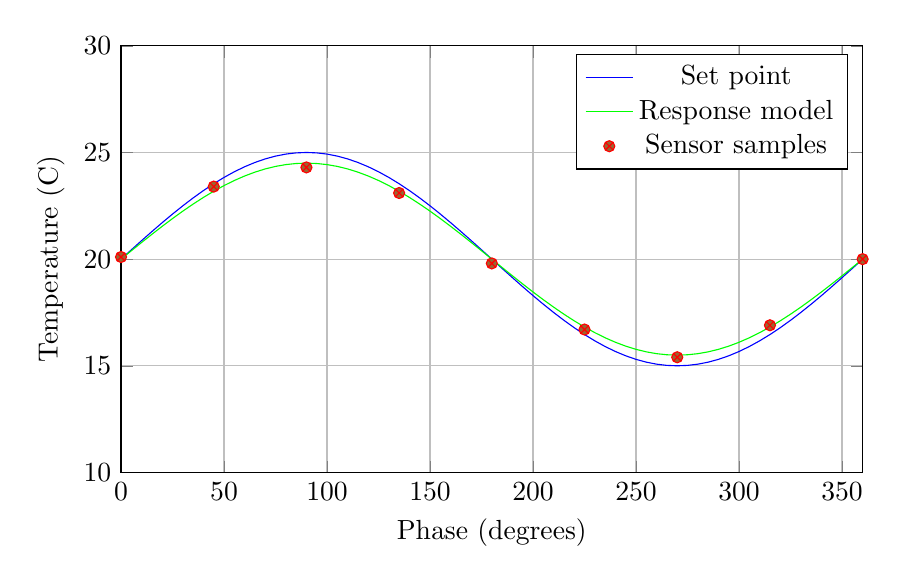
\begin{tikzpicture}
  \begin{axis}[
    xmin=0,xmax=360,ymin=10,ymax=30,
    width=11cm,height=7cm,
    xlabel={Phase (degrees)},ylabel={Temperature (C)},
    grid=major,domain=0:360,samples=73]
    \addplot[blue] {20+5*sin(x)};
    \addlegendentry{Set point}
    \addplot[green] {20+4.5*sin(x)};
    \addlegendentry{Response model}
    \addplot+[red,only marks] coordinates {
      (0,20.1) (45,23.4) (90,24.3) (135,23.1)
      (180,19.8) (225,16.7) (270,15.4) (315,16.9) (360,20.0)
    };
    \addlegendentry{Sensor samples}
  \end{axis}
\end{tikzpicture}
\caption{Set point, response model, and measured temperatures.}
\label{fig:thermal-cycle}
\end{figure}

The two smooth curves test degree-based trigonometric sampling, while the
red observations test point placement across the full domain.
\end{document}
